\chapter{Supplementary Results: Experiment A}
\label{appendix:expA}

\section{A2: 5--20\,MHz Band-averaged PSD per Laser Current}
\label{appendix:A2Table}
\autoref{tab:A2-band-psd} gives the data plotted in \autoref{fig:A2PSDvsCurrent}: the detector output PSD averaged over the 5--\SI{20}{\mega\hertz} band for each laser drive current with balanced detection. The laser-off (electronic) floor is \SI{8.061e-14}{\volt\squared\per\hertz}; the excess above this floor is taken as the shot noise $S$, and the last column gives the total noise $T$ relative to the shot-noise limit, $10\log_{10}(T/S)$, which performance requirement P1 requires to be $\leq \SI{1}{\decibel}$.

\begin{table}[H]
	\centering
	\small
	\begin{tabular}{@{}S[table-format=2.0] S[table-format=1.4] S[table-format=1.4] S[table-format=3.1] S[table-format=1.2] S[table-format=1.2]@{}}
		\toprule
		{Current} & {Total PSD $T$} & {Excess $S = T - E$} & {Voltage noise} & {$T/E$} & {$T/S$} \\
		{(mA)} & {($10^{-13}$ V$^2$/Hz)} & {($10^{-13}$ V$^2$/Hz)} & {(nV/$\sqrt{\text{Hz}}$)} & {(dB)} & {(dB)} \\
		\midrule
		7 & 1.1127 & 0.3066 & 333.6 & 1.40 & 5.60 \\
		11 & 1.3797 & 0.5736 & 371.4 & 2.33 & 3.81 \\
		15 & 1.8440 & 1.0379 & 429.4 & 3.59 & 2.50 \\
		23 & 2.8416 & 2.0355 & 533.1 & 5.47 & 1.45 \\
		31 & 3.6844 & 2.8783 & 607.0 & 6.60 & 1.07 \\
		38 & 4.6072 & 3.8011 & 678.8 & 7.57 & 0.84 \\
		48 & 5.2954 & 4.4893 & 727.7 & 8.18 & 0.72 \\
		\bottomrule
	\end{tabular}
	\caption{A2: band-averaged (5--\SI{20}{\mega\hertz}) detector PSD with balanced detection versus laser drive current. $E = \SI{8.061e-14}{\volt\squared\per\hertz}$ is the laser-off electronic floor.}
	\label{tab:A2-band-psd}
\end{table}


\section{A3: Supplementary Experiment on RIN Cancellation}
\label{appendix:RINValidation}
% Referenced from: Sec 4.2.1 and Sec 4.2.3 (A3 paragraph).
\autoref{fig:A3Plot} gives the 5 - 20MHz averaged PSD of the detected noise, when only a single photodetector input of the PD100B is used - effectively turning it into a singe-ended detector. The electronic noise floor will remain the same, but the total noise PSD averages will now also contain RIN in addition to shot-noise and electronic noise. Before analysis of this plot can commence, it is important to note that in the case of balanced detection, the shot-noise of each detector is uncorrelated, and will therefore add together at the output. Thus, in the single-ended case, the shot-noise at the output for a given laser current is expected to be half that of the balanced detection case. Any excess noise above this half-power shot-noise level is thus contributed from the electronic noise, and the uncancelled RIN.

\begin{figure}[H]
	\centering
	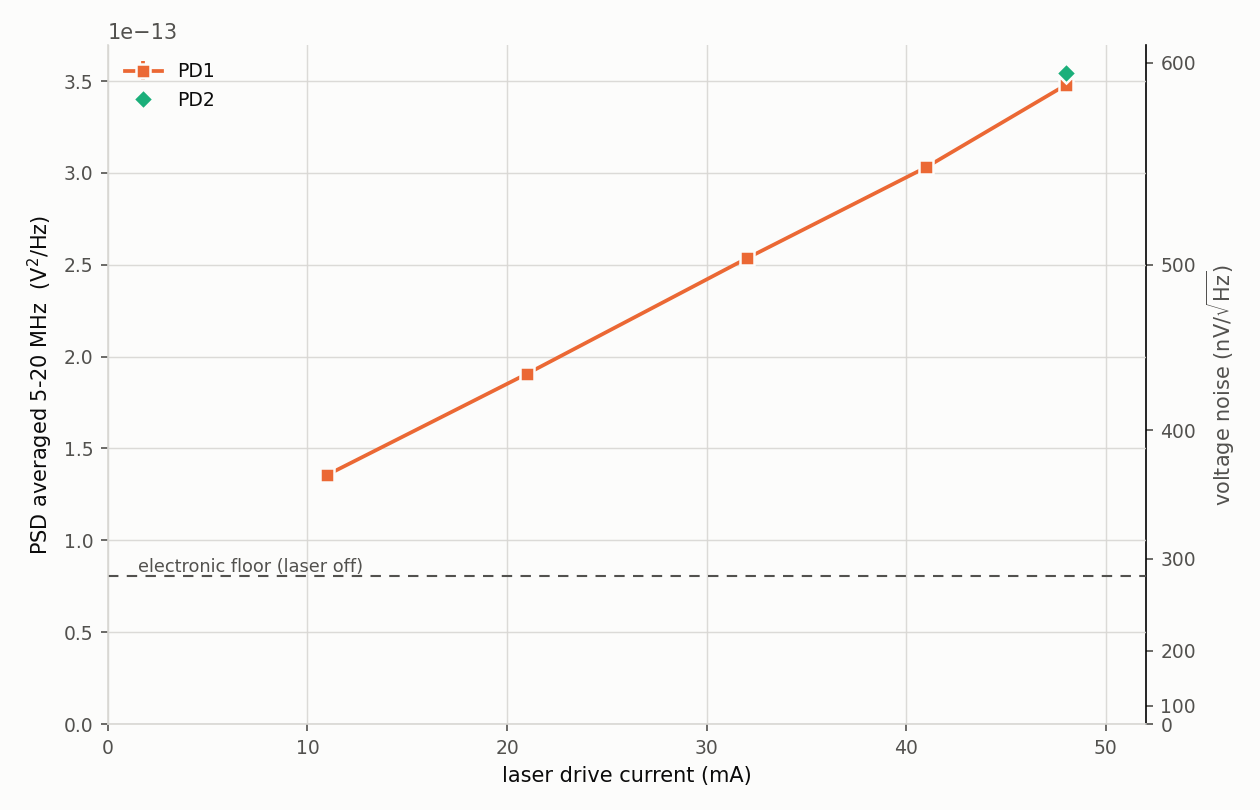
\includegraphics[width=1\linewidth]{psd_vs_current_single.png}
	\caption{A3: 5 - 20MHz Average PSD vs Laser Current with Single-Ended Detection}
	\label{fig:A3Plot}
\end{figure}

It can be seen in \autoref{fig:A3Plot} that indeed, the total noise is lower than in \autoref{fig:A2PSDvsCurrent}, as expected. Observing the total noise at the operating point of 48mA however, it can be seen that a value of approximately $3.5 \times 10^{-13}V^2/Hz$ is obtained, which gives $2.694\times 10^{-13}V^2/Hz$ once electronic noise has been subtracted. In the balanced detection case at the same laser current, a value of $5.2954\times10^{-13}V^2/Hz$ was obtained - subtracting electronic noise and halving this gives $2.245\times 10^{-13}V^2/Hz$. This clearly indicates that the noise power in the single-ended case is higher than simply half of the shot-noise in the balanced detection case, thus proving that indeed there is excess RIN present. This excess RIN noise can be calculated:
\begin{equation}
	RIN_{excess}= (2.694 - 2.245)\times 10^{-13} = 0.449\times 10 ^{-13}V^2/Hz
\end{equation}

Converting to dB:

\begin{equation}
	10log_{10}(1+\frac{RIN_{excess}}{S})=10log_{10}(1+\frac{0.449\times 10 ^{-13}}{2.245\times 10^{-13}})= 0.79dB
\end{equation}

Thus, RIN contributes an additional 0.79dB of noise above the ideal shot-noise limit at the 48mA operating point. Balanced detection allows this excess noise to be removed, as illustrated in the results of A2 - allowing for a better SNR.


